\chapter{Moodle}
\label{cha:moodle}

Moodle to darmowy open-sourcowy program służący do zarządzania kursami uczelnialnymi. System jest napisany w PHP i dytstrybuowany pod licencją GNU. Stworzony z pedagogicznych pobudek, Moodle jest używany do różnorakiej nauki, zdalnej edukacji. Wykorzystując dostosowywalne zarządzanie opcjami, moodle jest używany do tworzenia prywatnych stron oferujących kursy internetowe dla trenerów oraz nauczycieli. Moodle ( akronim od Modular Object-Oriented Dynamic Learing Environment) pozwala na rozszerzanie i dopasowywania środowiska, wykorzystując szeroko dostępne w społeczności pluginy.

Struktura Moodle jest klasyczna dla portalu wymagającego posiadania kont. W Moodle każdy użytkownik posiada osobne konto, do którego przypisana jest jakaś rola. Rolą może by np. administrator, prowadzący kurs albo uczestnik. Żeby stworzyć konto należy się zarejestrować. Moodle jest napisany w całości w PHP, wykorzystuje serwer Apache oraz bazę danych PostgreSQL.

W naszych testach zajęliśmy się aplikacją webową Moodle. Jest to platforma e-learningowa pozwalająca na publikację treści szkoleniowej, do tego jest ona wielopłaszczyznową platformą umożliwiającą aktywny kontakt między użytkownikami, a osobami definiującymi treść.

Moodle oferuje nam możliwość pracy w trzech trybach użytkowników takich jak:
\begin{itemize}
\item Nauczyciel – ma możliwość definiowania kursów oraz testów ustalania progów zdawalności, dodawania uczestników kursu, wysyłania komunikatów, określania sposób dostępu do kursu (otwarty, wymagane hasło dostępowe),
\item Uczeń/student – uczestnictwo w kursach, pobieranie zamieszczanych materiałów dydaktycznych, uczestnictwo w kursach, możliwość uzupełniania ankiet, egzaminów
\item Administrator – możliwość definiowania kursów oraz testów, zarządzanie sposobem dostępu do platformy, budowanie głównego layoutu platformy, definiowanie ról i uprawnień, zarządzanie platformą, generowanie raportów i zestawie
\end{itemize}
Poniżej dołączyliśmy zrzuty z testowanej aplikacji Moodle:

\noindent
\begin{minipage}{\linewidth}
\makebox[\linewidth]{
  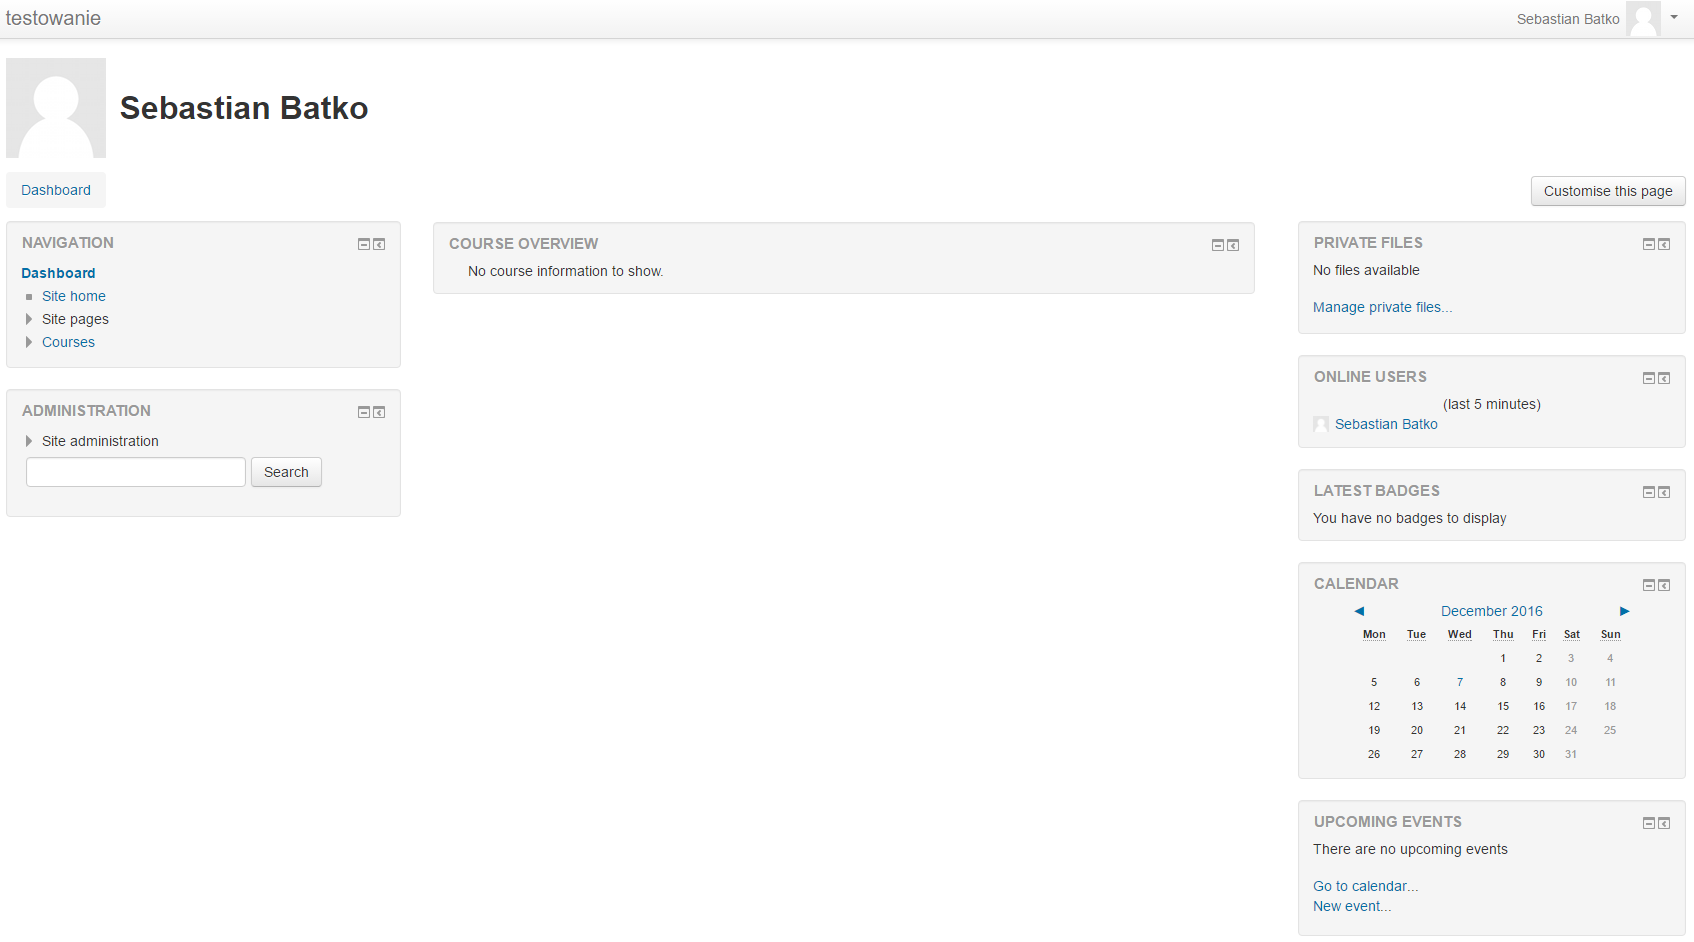
\includegraphics[keepaspectratio=true,scale=0.3]{pictures/moodle.png}}
\captionof{figure}{Moodle - panel główny}\label{erd}
\end{minipage}

\noindent
\begin{minipage}{\linewidth}
\makebox[\linewidth]{
  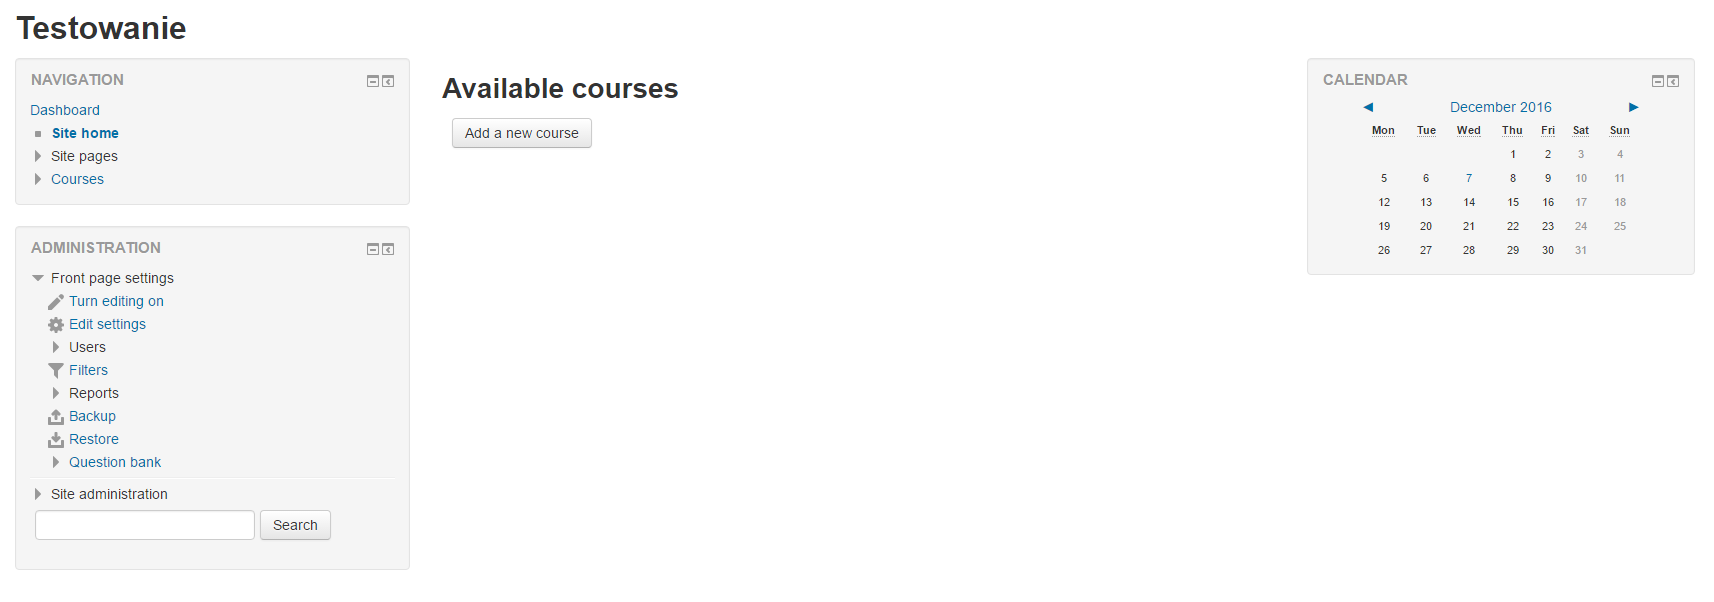
\includegraphics[keepaspectratio=true,scale=0.3]{pictures/moodle2.png}}
\captionof{figure}{Moodle - dostępne kursy}\label{erd}
\end{minipage}
